\documentclass{TISE}

% additional packages
\usepackage{etoolbox}
\usepackage{float}
\usepackage{soul}
\usepackage{amsfonts}
\usepackage{makecell}

\renewcommand\theadalign{bc}
\renewcommand\theadfont{\bfseries}
\renewcommand\theadgape{\Gape[4pt]}
\renewcommand\cellgape{\Gape[4pt]}

\graphicspath{{figures/}}

% title info
\title{Not just normal: Exploring power with Shiny apps}
\author{Removed for blinding}

\begin{document}
	
\pagenumbering{roman}
\setcounter{page}{3}

\begin{abstract}
	Statistical power taught in most graduate-level and undergraduate-level mathematical statistics courses, but is difficult to understand conceptually. Visualizations of the power curve, sampling distributions, and how they interact can help students understand power, but creation of such visuals can be difficult and time-consuming. Interactive web applications provide a way for students to dynamically visualize power, and many web applications for understanding power exist. However, most of these applications assume samples are drawn from a Normal population, concern only the sample mean, and/or were created for introductory classes. In this paper, we describe a web application suitable for undergraduate-level and graduate-level mathematical statistics classes that we created to allow users to visualize the complex relationships underlying power for multiple different statistics and population distributions (available at \url{https://powerapp.shinyapps.io/powerapp/}); source code is provided for instructors who wish to modify the application. We also discuss our experience implementing this application across three different semesters, providing example activities in the appendix.  
\end{abstract}
	
\section{INTRODUCTION}

Statistical power is a fundamental component of most graduate-level and undergraduate-level mathematical statistics courses, and yet it is frequently cited as one of the most difficult topics to teach \citep{aberson2002}. This difficulty is driven by the conceptual richness of the topic. To fully understand power, students must understand the relationship between the sampling distributions of the test statistic across both the null and alternative parameter spaces and how they are used to compute power, as well as the factors that influence those distributions. Guiding students towards a conceptual understanding of these relationships can be challenging, as the relationships are difficult to visualize using traditional classroom methods \citep{aberson2002}.

In traditional upper-level mathematical statistics courses, such as curricula based on \citet{wackerly2008} or \citet{casella2002}, power is typically explored through its definition and derivations of power functions. \cite{casella2002} define power by considering a hypothesis test of $H_0 : \theta \in \Theta_0$ versus $H_1 : \theta \in \Theta_0^c$ and defining $\mathcal{R}$ as the rejection region for that test. They then define the power function of this test as $\beta(\theta) = P(\boldsymbol{X} \in \mathcal{R} | \theta)$. In words, the power function represents the probability of rejecting the null hypothesis for a given value of $\theta$. \cite{casella2002} follow this definition with derivations of the power function for samples from the binomial and normal population distributions, respectively. This method of presenting and exploring statistical power - largely through computational mechanics - is mirrored in many of the traditional curricula based on this text. 

From the definition and derivation of a hypothesis test's power function, students are expected to understand a range of learning objectives. Potential learning objectives for power include but are not limited to:
\begin{itemize}
	\item[1)] understanding how the sample size, null value, alternative hypothesis, significance level, test statistic, and population distribution each affect power;
	\item[2)] understanding the relationship between the power function and the sampling distribution of the test statistic under both the null hypothesis and the true value of $\theta$; and
	\item[3)] understanding how to calculate the power of a hypothesis test using a variety of strategies.
\end{itemize}

However, students' conceptual understanding of complex topics such as power can be enhanced by the use of graphical and visualization techniques (\citealt{delMas1999}; \citealt{chance2007}; \citealt{bobek2016}). The \textit{Guidelines for Assessment and Instruction in Statistics Education} (GAISE) report promotes using technology to visually represent complex introductory statistics concepts \citep{ASA2016}, and the \textit{2014 Curriculum Guidelines for Undergraduate Programs in Statistical Science} \citep{ASA2014} extend these expectations to undergraduate statistics courses in general, placing renewed vigor on developing undergraduate statistics curriculum that allow students to develop a conceptual understanding of the material and think critically. \cite{wild2011} describe how technology can be used to ``change the landscape of statistics education," (p. 248) due to its ability to allow students to conceptualize in ways unavailable in its absence. \cite{green2015} describe various tools that can be used to foster active learning and conceptual understanding of the concepts discussed in a traditional mathematical statistics curriculum; among these tools is the use of technology and visualizations. 

To create visualizations that allow students to develop a conceptual understanding of power, students must first derive multiple power functions - for differing population distributions, statistics, and alternative hypotheses - and then plot the functions using statistical software. Although there is value to each of these steps, the time commitment and difficulty of the task may frustrate students and distract from understanding the learning objectives. Alternatively, instructors may create graphics either during class in real-time or in advance. The former case requires substantial coding experience on the part of the instructor and demands class time, and the latter case can be restrictive in that students cannot organically explore factors that affect the power function as the visuals were created by the instructor in advance.

Alternatively, instructors may used web-based applications when teaching power that allow students to make interactive discoveries using point-and-click graphical interfaces. Using such applications lets students interactively explore graphical representations of power without having to first create those visualizations. Many graphical tools for understanding statistical power exist (\citealt{aberson2002}; \citealt{andersoncook2003}; and \citealt{rossman2004}; \citealt{post2016}), but most assume samples are drawn from a normal population and were created for introductory courses. To offer other options, instructors may either adapt a currently existing application, which requires access to source code and literacy in the source coding language, or develop one of their own, which requires considerable time and knowledge of many different coding languages \citep{doi2016}.  

We desired a web application that allows students to explore what factors affect the power function for many different test statistics assuming population distributions beyond the normal distribution. Additionally, we wanted students to be able to visualize and interactively explore both the power function and the sampling distributions of the test statistic over the null and alternative parameters spaces. These goals motivated the development of our web application, offering a flexible tool other instructors can use to teach power. In this article we discuss how the layout and features of the application are designed to help promote students' conceptual understanding of power through the use of visualizations. We then describe how this web application can be used to address the learning objectives provided above and share our experience using it in undergraduate and graduate-level mathematical statistics courses. Finally, we conclude with a discussion of the value of this web application and opportunities for future work. 

\section{APPLICATION LAYOUT}

When designing this web application, we had two primary goals. First, we wanted to develop a tool that allows students to visualize the relationship between the power function and various factors that influence it. In particular, we wanted students to be able to explore the effect of the population distribution, statistic of interest, null value, alternative hypothesis, significance level, and sample size on the power function in real time without needing to derive or plot that function. We also wanted students to visualize the relationship between the power function and the sampling distribution under both the null hypothesis and true value of theta to develop a conceptual understanding of how power is derived. The development of such a web tool provides an efficient way to support students' conceptual understanding of power and sampling distributions through visualizations without spending class time creating them. These goals led to the development of the {\sf R} Shiny application provided in \hl{Figure 1}. 

This web application features three different families of population distributions: the exponential($\theta$) family, the normal($\theta$, $\sigma^2$) family, and the uniform(0, $\theta$) family of distributions. For any population distribution, three statistics are available: the sum of the random variables, the sample minimum, and the sample maximum. For each combination of population distribution and statistic, there are three alternative hypotheses available: a not equal to alternative, a greater than alternative, and a less than alternative. The user also has the option to specify the sample size, significance level, and null value. Based on these options, the power curve is plotted in the main plotting window. Beneath that, the sampling distribution of the statistic under both the null hypothesis and true value of $\theta$ is plotted once the respective point on the power curve is clicked. 

\newpage

\begin{figure}[H]
	\centering
	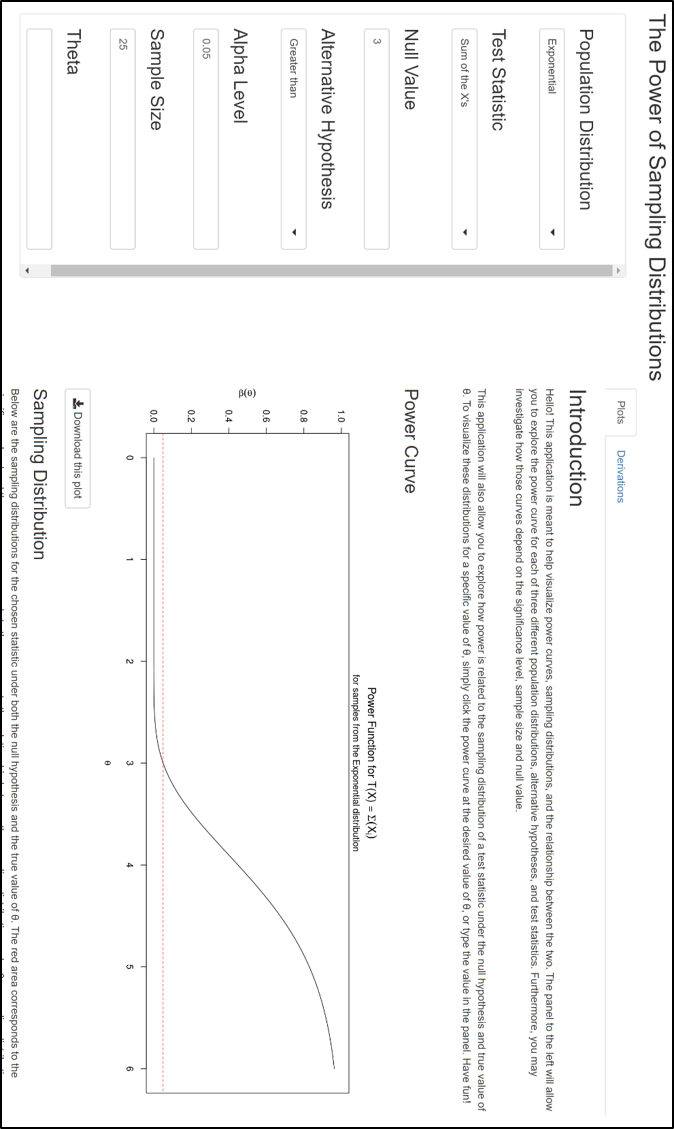
\includegraphics[scale=1]{app_layout.png}
	\caption{Interface for the web application. In the side panel, users may specify the population distribution, test statistic, null value, alternative hypothesis, significance level, and sample size. Based on these selections, the power curve is created in the main plotting window in real time.}
\end{figure}

We chose to create this application in {\sf R} Shiny because of its use of reactive programming. Reactive programming allows the application to tailor output based on user input in real time. This is particularly useful when exploring power as it allows users to investigate the relationship between the power curve and sampling distribution of the statistic in an interactive way. In this web application, the user is able to visualize the sampling distribution of the statistic for a particular value of $\theta$ by either clicking on a point on the graph of the power function or by specifying the value in the ``Theta" box on the side panel (\hl{Figure 2}). Note that this plot is not visible until $\theta$ is specified using one of these two options. Additionally, both plots respond in real time to any changes in the options provided on the side panel. This allows users to quickly assess the impact of any of those changes on both the power function and the sampling distributions, thereby helping them understand the relationship between the options on the sidebar, the power function, and the sampling distributions. 

\begin{figure}[H]
	\centering
	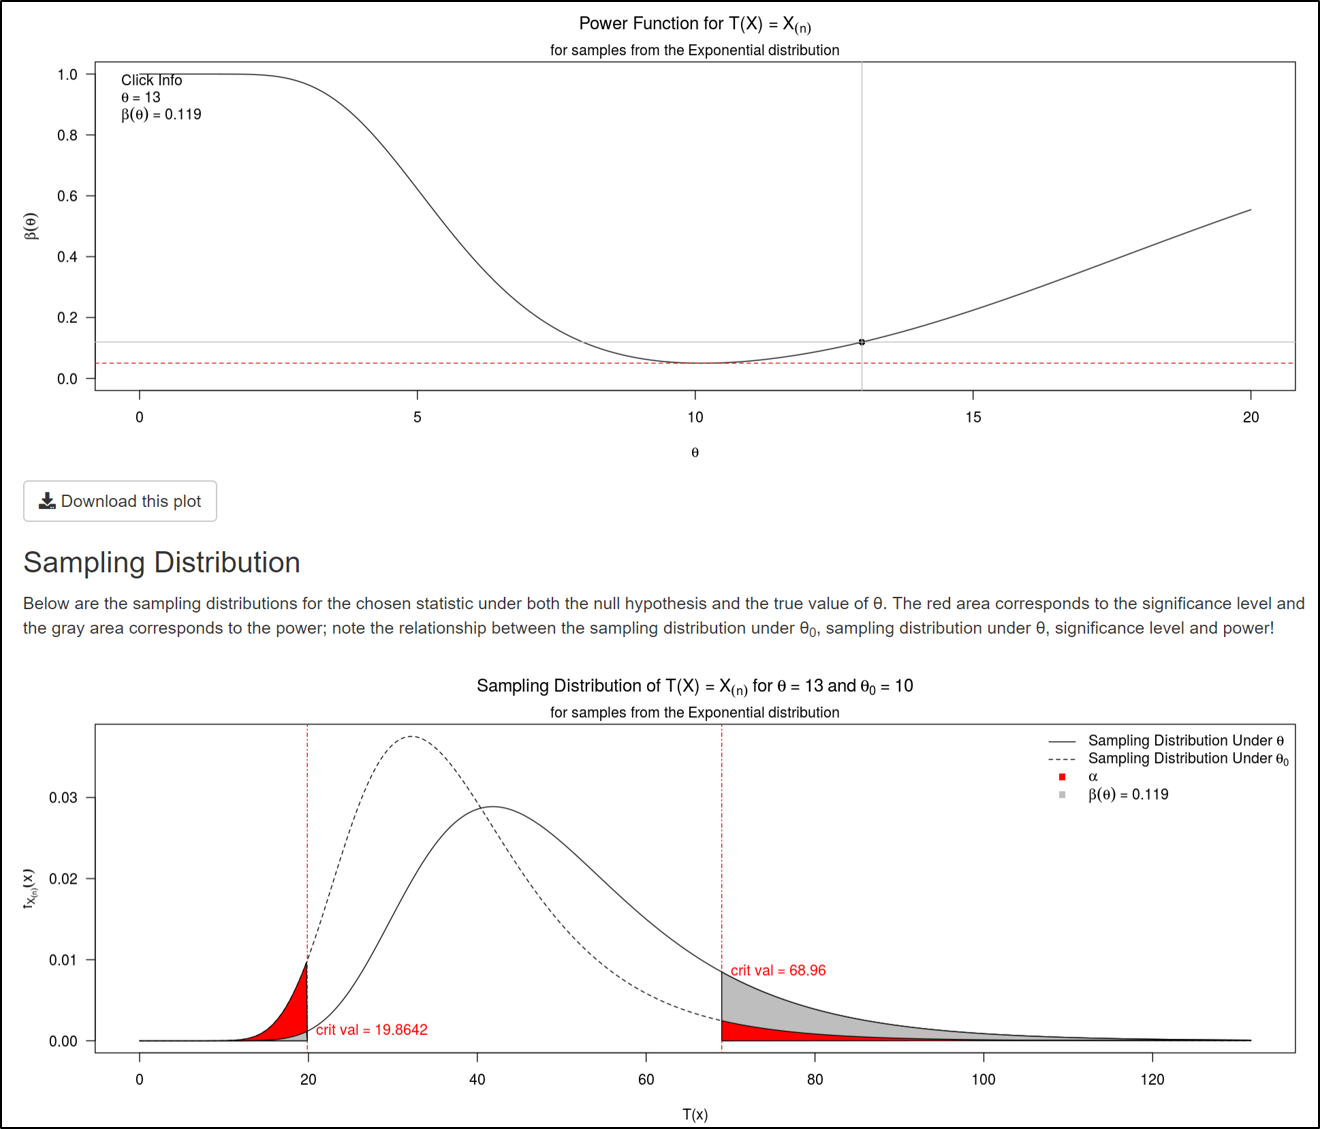
\includegraphics[scale=1]{reactive2.png}
	\caption{Power function for a hypothesis based on the sample maximum for a sample of size 25 from the exponential distribution assuming a not equal to alternative hypothesis, significance level of 0.05, and null value of 10. The sampling distribution plot is created once a point on the power curve is selected and updated in real time based on any subsequent changes to inputs on the side panel or theta.}
\end{figure}

We compartmentalized many of the features of this application to allow users to focus on specific topics rather than other potentially distracting features. For example, the conditionality of the sampling distribution plot allows users to explore relationships between the options on the sidebar and the power function before considering sampling distributions. In addition, this web application presents distribution specific options. For example, specification of the population standard deviation, $\sigma$, is only available when the normal distribution is selected. A host of other options appear when both the uniform distribution and sum of random variables are selected, allowing the user to explore the numerical instability present in the distribution function associated with that statistic when sampling from the uniform distribution (see Section 3.3 for discussion). By consciously hiding certain options and tabs when they are not needed, the user is able to focus on learning without added distractions. 

\begin{figure}[H]
	\centering
	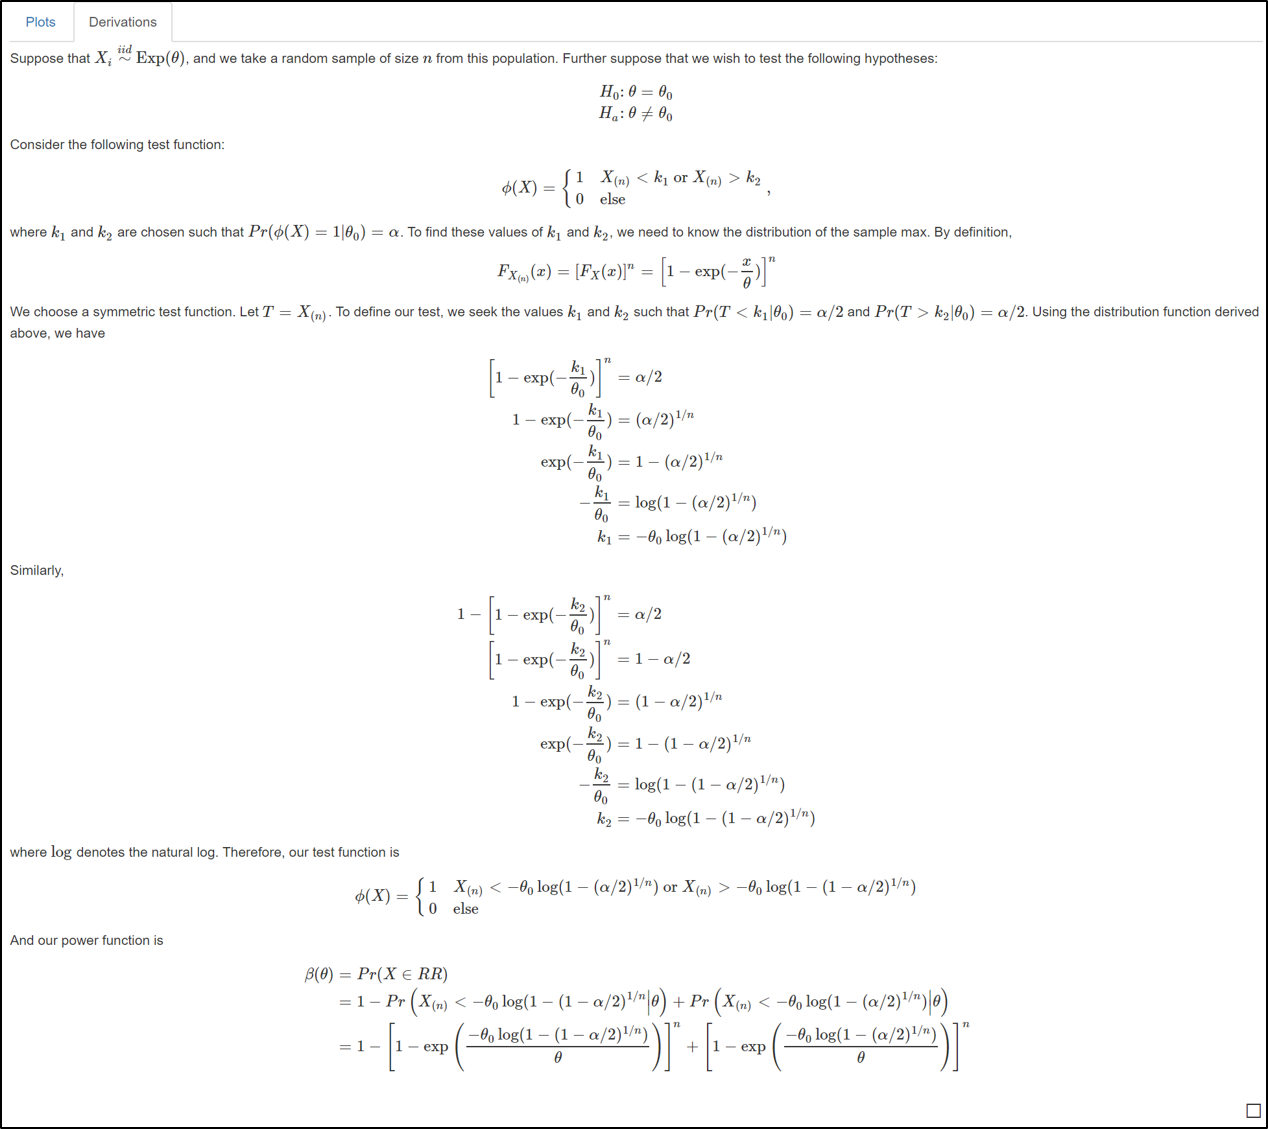
\includegraphics[width=\linewidth]{derivs.png}
	\caption{Power function derivations for a hypothesis test based on the sample maximum for samples drawn from an exponential population assuming a not equal to alternative hypothesis. The population distribution, test statistic, and alternative hypothesis are selected using a sidebar panel (not pictured).}
\end{figure}

In addition to these structural features, we included features to make the application more user friendly, including  download options for each of the created plots and tabs to work through the derivations of each power curve. The download option supports easy sharing and collaborative explorations within a classroom. For example, in our experience students were asked to investigate a particular relationship (e.g., the relationship between sample size and the power function) and upload images supporting their findings to a shared Google document which was then used for class discussion. If desired, the derivations tab allows users to work through the derivations for each of the power functions provided in the plots tab (\hl{Figure 3}). Although the focus of this application is on developing understanding through visualizations, we included the derivations to help users build connections between the graphical and mathematical representations of power.

This web application was consciously designed to support students' learning of power through the reactive nature of Shiny, our choice to compartmentalize application features, and several user friendly additional features. In the next section, we discuss how this conscious design can be used to address each of the learning objectives provided in Section 1.

\section{APPLICATION EXPLORATIONS}

An advantage of teaching power through this web application is that it allows for creativity and flexibility in how the instructor approaches the topic. Through tabular panels and conditional plots, this applet lets instructors choose which aspects of power to focus on, while still allowing students to explore at their own pace. In this section, we describe how this applet may be used to explore the learning objectives defined in Section 1. Section 3.1 focuses on power curves and how they change for different population distributions, test statistics, null values, alternative hypotheses, alpha levels, and sample sizes; Section 3.2 focuses on how those curves arise by examining sampling distributions of test statistics under a number of different conditions; and finally, Section 3.3 explores alternatives to traditional methods of determining power.

\subsection{Exploring power curves}

Statistical power is a complex concept that is influenced by several factors, including the distribution from which one is sampling, the statistic chosen to summarize the sample, the hypothesis of interest, the significance level, and the number of observations drawn from the population. As noted in Section 1, these relationships are often examined through the derivation of a power curve, but students' conceptual understanding of these relationships can be greatly enhanced through the use of visualizations. Creating these visualizations requires fluency in a coding language and mathematical expertise, as well as class time to create them. 

The use of this web application can help alleviate these requirements by allowing students to visualize relationships between the power curve and a host of different factors without having to derive the power function and code required to plot that function. For the remainder of this section, we highlight how this applet may be used to make connections between the power curve and each of those factors.

\subsubsection{Varying the population distribution}

The role of the population distribution in a power function is one of the more abstract relationships we consider in this application, as it only manifests through the functional form of the power function. Consequently, it can be a difficult topic to explore without visuals. This web application provides an easy way to explore this relationship as it allows the user to quickly switch between population distributions while holding the statistic, null value, alternative hypothesis, significance level, and sample size constant. Students can be guided through this exploration by asking them to fix a particular combination of these factors while varying the population distribution of interest. For example, \hl{Figure 4} provides a suite of plots for a hypothesis test based on the sample maximum with a greater than alternative hypothesis, a null value of 3, a significance level of 0.05, and a sample size of 25 from three different population distributions.

\begin{figure}[H]
	\centering
	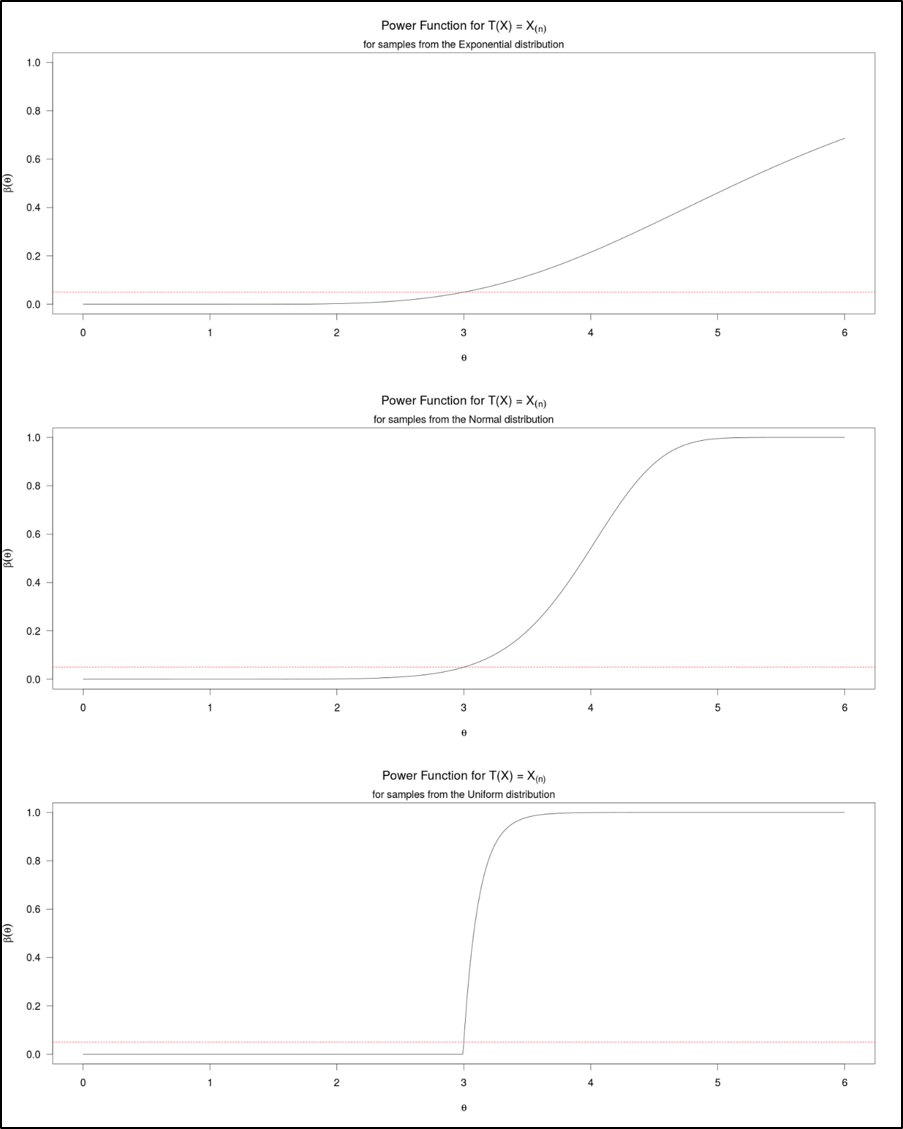
\includegraphics[height=4in,width=4in]{varypop.png}
	\caption{Comparison of the power function for the sample maximum from each of the exponential (top), normal (middle), and uniform (bottom) distributions.}
\end{figure}

Using \hl{Figure 4} or another example, students can compare how quickly each of the power functions are increasing as $\theta$ increases and discuss how and why these differences arise. Students must understand what $\theta$ represents in each of these populations, as well as what a power function represents at each value of $\theta$, which is a fundamental learning objective when considering power. Students may also be prompted to discuss which power function is closest to an ideal power curve. To answer such a question, students must first consider what an ideal power function looks like for the alternative hypothesis of interest, which further reinforces their understanding of what a power function represents at each value of $\theta$. Addressing this question also entails considering the behavior of the power function over both the null and alternative parameter spaces, and how that behavior relates to the alternative hypothesis. Following these questions, students may be asked to brainstorm what other factors might affect the power function, each of which may be explored by varying other options on the web application.

\subsubsection{Varying the test statistic}

In standard mathematical statistics courses based on textbooks, such as \cite{casella2002}, students are often asked to use power curves to compare test functions based on different test statistics. In the web application, students can make such comparisons by providing a specific combination of factors in the side panel of this web application. For example, \hl{Figure 5} provides a set of plots comparing each of the available statistics for the uniform and normal population distributions (assuming a null value of 3, significance level of 0.05, not equal to alternative hypothesis, and sample size of 25).

\begin{figure}[H]
	\centering
	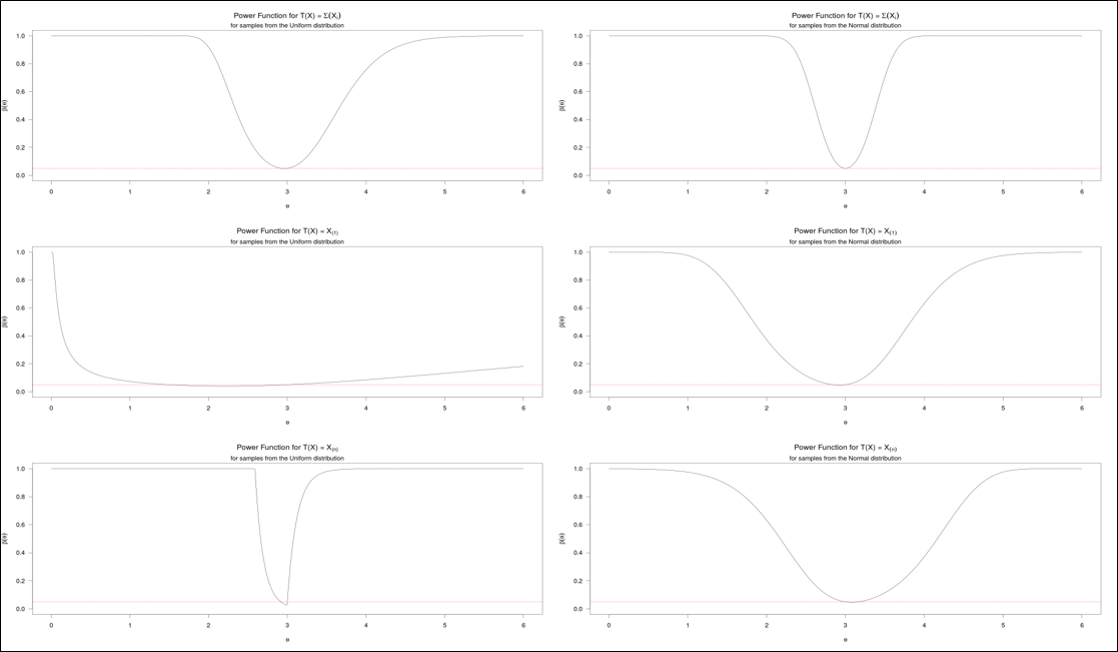
\includegraphics[height=4.5in, width=6in]{varystat.png}
	\caption{Comparison of power functions for varying statistics and population distributions. The left and right columns correspond to samples from the uniform and normal distribution, respectively. The top, middle, and bottom rows correspond to test functions based on the sum of random variables, sample minimum, and sample maximum, respectively.}
\end{figure}

From \hl{Figure 5}, students may be asked to identify which power function is closest to ideal for each population distribution. This question helps students understand that the test statistic that provides the highest power in the alternative space depends upon the population distribution of interest. By choosing this particular combination of statistics and population distributions, students may be asked to think critically about why the sum of random variables performs best for the normal distribution and why the sample maximum performs best for the uniform distribution. This avenue of exploration can lead to discussions of sufficiency in the context of power thereby helping students draw connections between power and previously explored topics.  

\subsubsection{Varying the alternative hypothesis}

This web application can also be used to help students understand the effect of the alternative hypothesis on the power curve. Varying the alternative hypothesis while holding all other aspects of the power curve constant allows students to consider the relationship between the null and alternative parameter spaces and what the power function represents across each of these spaces. For example, \hl{Figure 6} showcases this exercise for a hypothesis test based on the sum of random variables for samples of size 25 from the exponential distribution. 

\begin{figure}[H]
	\centering
	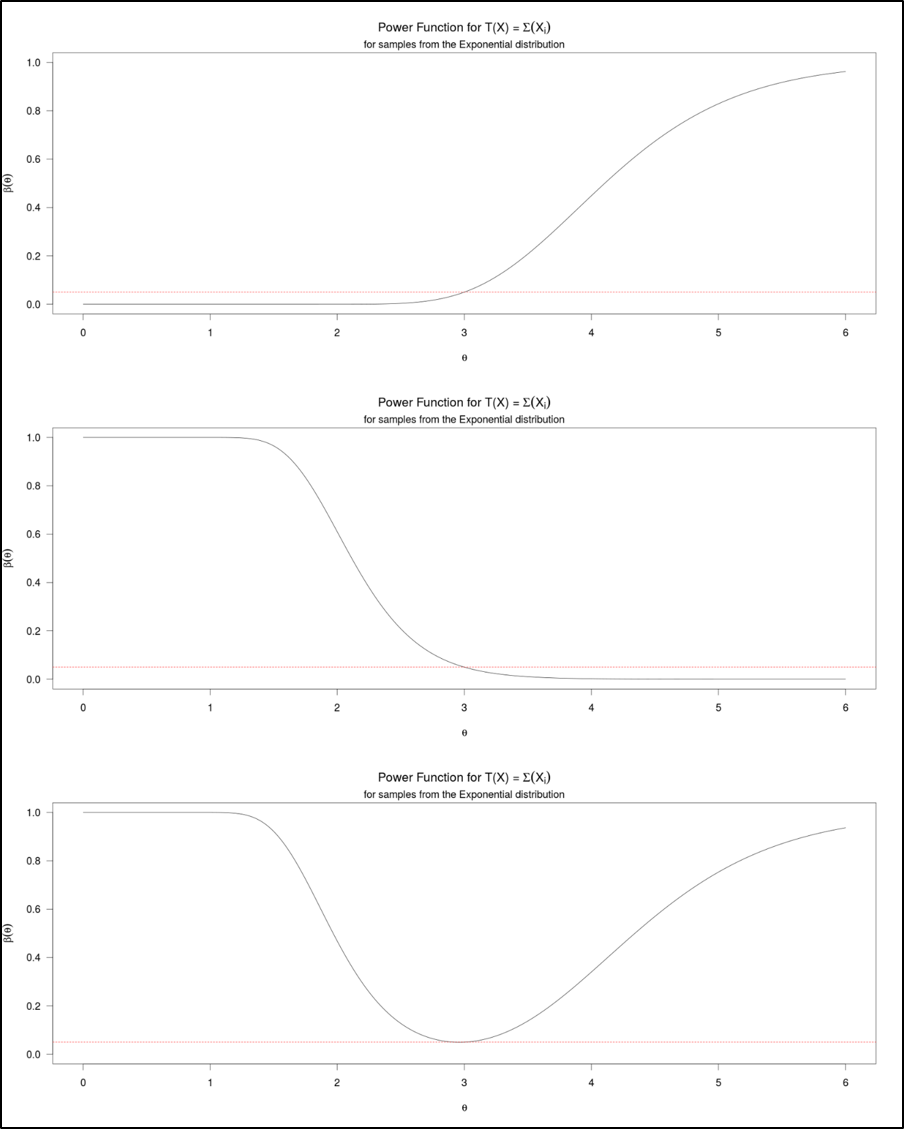
\includegraphics[height=4in,width=4in]{varyalt1.png}
	\caption{Comparison of alternative hypotheses for hypothesis tests based on the sum of random variables when sampling from the exponential distribution. The top row corresponds to a greater than alternative, while the middle and bottom represent a less than and not equal to alternative, respectively.}
\end{figure}

Based on \hl{Figure 6}, students may easily visualize the effect of the alternative hypothesis on a power function; namely that for well-behaved tests, we expect greater power over the alternative parameter space than over the null parameter space. Students can also be asked to consider bias in a testing context by guiding them to look at the power function for the sample maximum from the uniform distribution (\hl{Figure 7}). This power function provides an example of an unbiased test, which is rarely discussed in depth in a traditional mathematical statistics course. 

\begin{figure}[H]
	\centering
	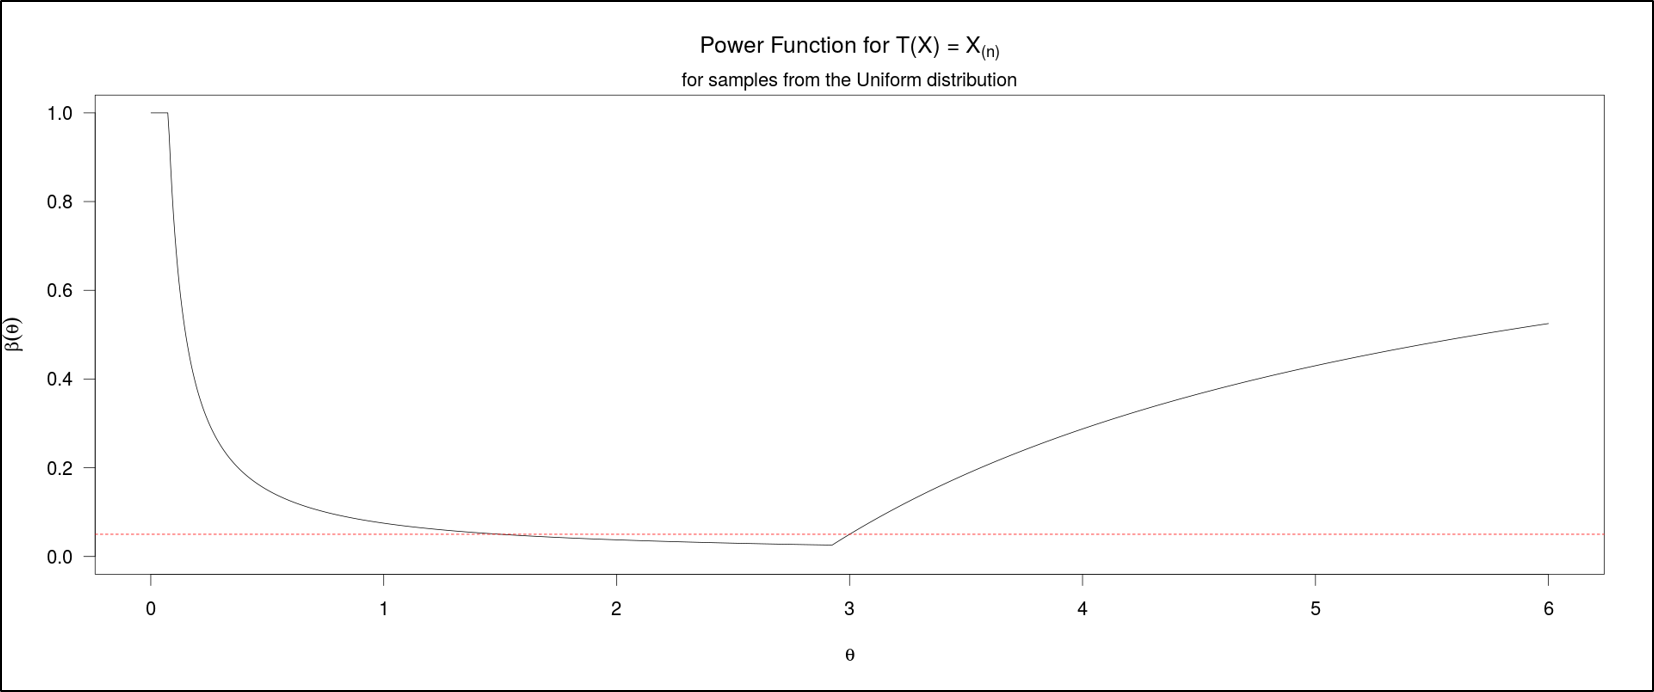
\includegraphics[width=\linewidth]{varyalt2.png}
	\caption{Power function for a hypothesis test based on the sample maximum assuming a sample of size one is taken from the uniform distribution with a not equal to alternative hypothesis.}
\end{figure}

This example is particularly interesting as the test is based on a complete, sufficient statistic and yet is biased. This apparent dichotomy motivates students to consider the advantages and disadvantages that may come with choosing certain statistics in different testing situations, offering rich classroom discussions. 

\subsubsection{Varying the significance level and null value}

The significance level plays a key role in deriving power as it is used to determine the critical values of a hypothesis test and also represents the type I error rate. To help students understand how the significance level and null value are used to define a hypothesis test, students may be asked to vary the significance level and null value while leaving the other factors on the sidebar of the web application constant. \hl{Figure 8} depicts this exercise with an exponential population. 

From the plots in \hl{Figure 8}, students can visually determine that for size $\alpha$ tests, the power of the test at the null value is equal to the significance level. They can also see that larger significance levels lead to greater power over both the null and alternative parameter spaces. Visualizing how the significance level and null value relate to one another and affect the power function may help students better understand how to derive a test function. 

In addition, students can consider more abstract relationships, such as the relationship between the power of a test and the type I error rate. Because the significance level is the maximum type I error rate over the null parameter space for a size $\alpha$ test, a compromise must be made between increasing the power of the test across the alternative parameter space and increasing the type I error rate when determining the appropriate significance level for a test. This compromise is easy to visualize from the plots displayed in \hl{Figure 8}, providing an opportunity for students to discuss the responsibility of the researcher in hypothesis testing.

\begin{figure}[H]
	\centering
	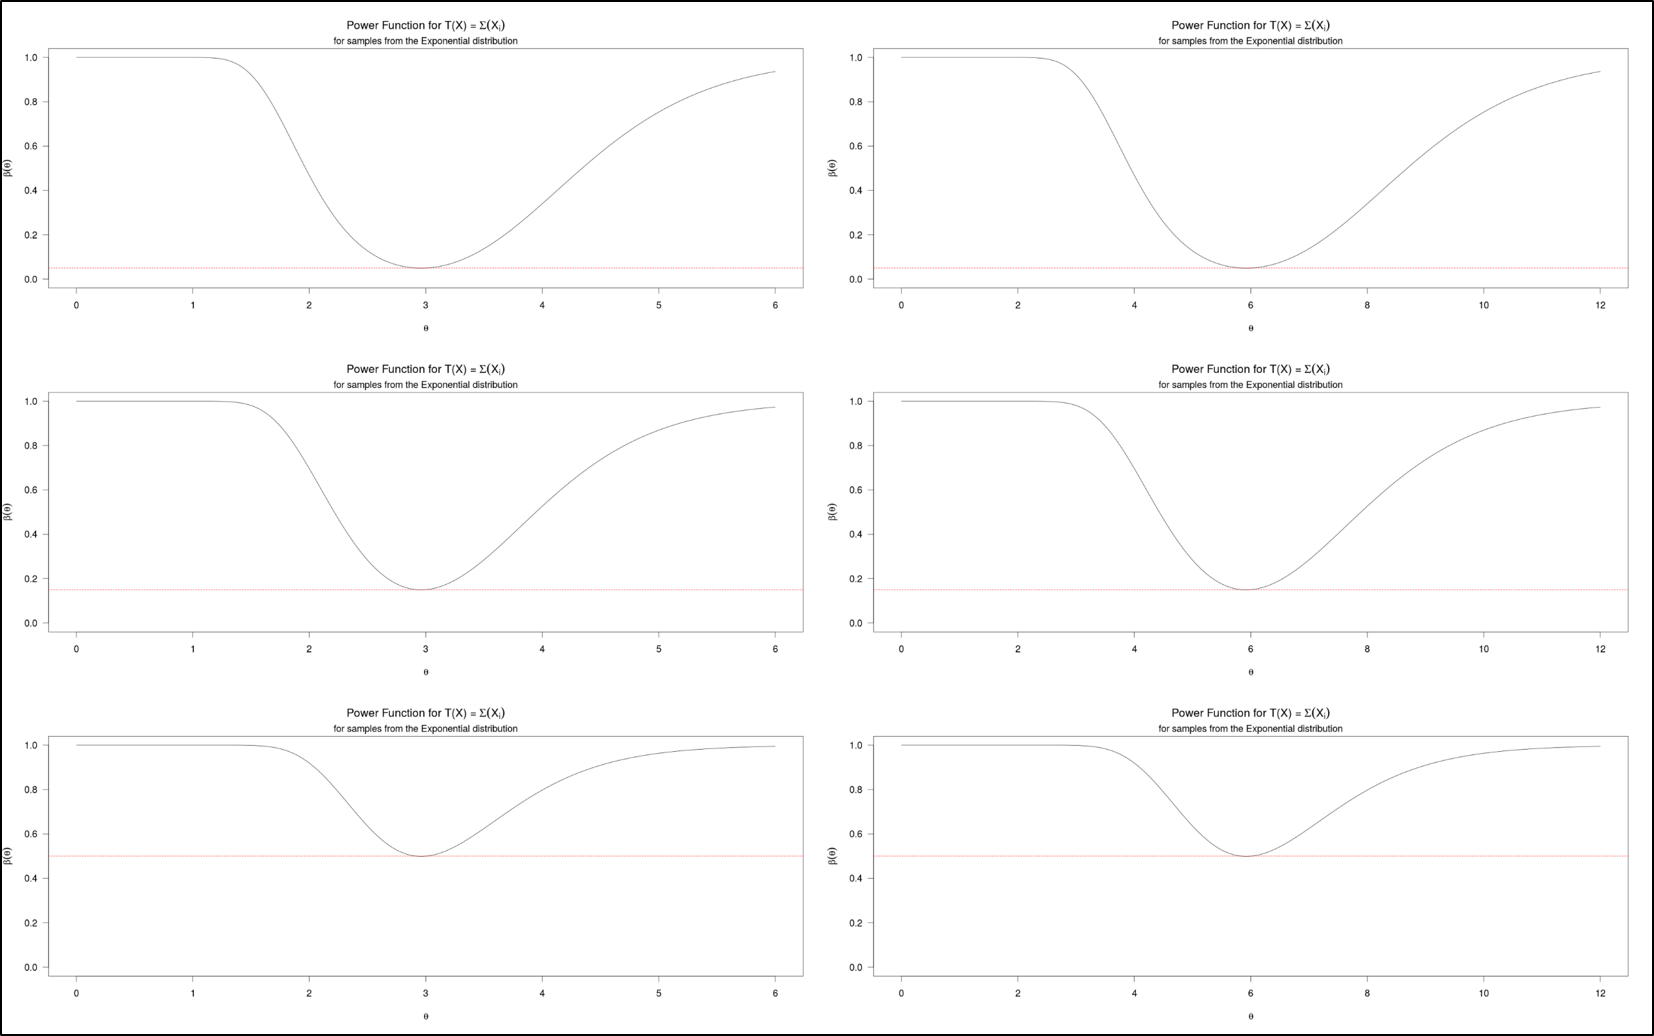
\includegraphics[width=\linewidth]{varyingsig.png}
	\caption{Comparison of power functions for varying significance levels and null values for hypothesis tests based on the sum of random variables for samples of size 25 from the exponential distribution. The left and right columns correspond to null values of three and six, respectively. The top, middle, and bottom rows correspond to significance levels of 0.05, 0.15, and 0.5 respectively.}
\end{figure}

\subsubsection{Varying the sample size}

Sample size is often another factor of interest when conducting power analyses. In general, as the sample size increases, so too does the power over the alternative parameter space. To help students understand this relationship, they may be asked to vary the sample size while holding all other factors constant. As an interesting example, \hl{Figure 9} depicts this exercise for both the sum of random variables and the sample minimum when sampling from a normal distribution. 

From these plots, students may easily determine the effect of the sample size on the power function. The plots also provide an opportunity to discuss why the sample size has a greater effect on the power function for the sum of random variables than it does on the power function for the sample minimum. Such a discussion requires students to consider why it is easier to determine that $\theta$ differs from the null value when considering a sum of normal random variables than when considering the sample minimum for a given sample size. In doing so, students must contemplate the sampling distribution of each statistic, as discussed further in the next section.

\begin{figure}[H]
	\centering
	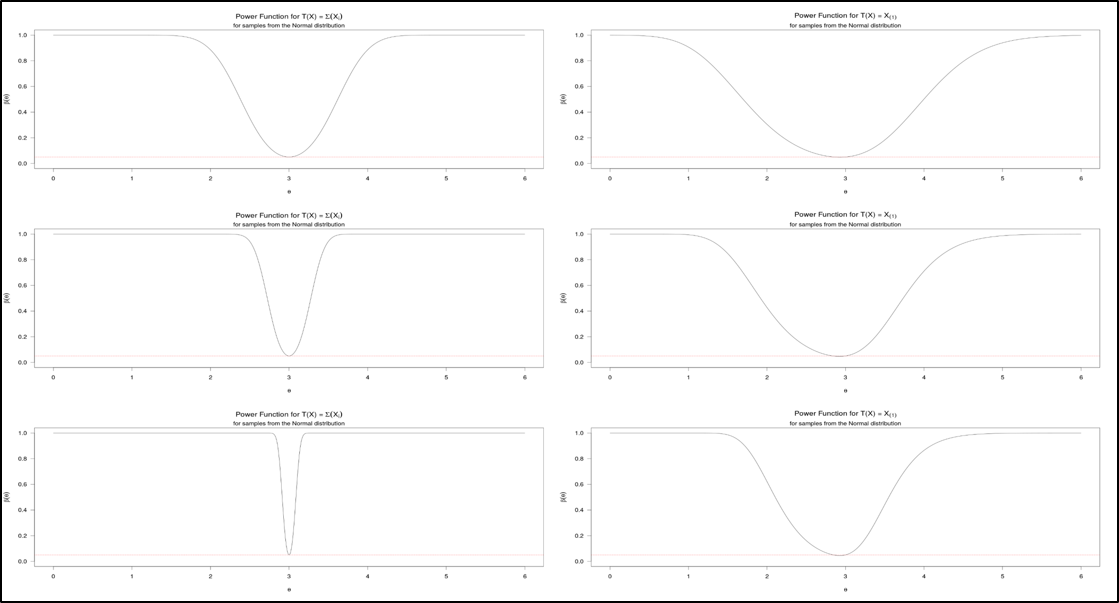
\includegraphics[width=\linewidth]{varyingn.png}
	\caption{Comparison of power functions for varying statistics and sample sizes for samples of size 25 from the normal distribution assuming a not equal to alternative hypothesis. The left and right columns correspond to the sum of the random variables and the sample minimum, respectively. The top row corresponds to a sample size of 10, the middle row to a sample size 50, and the last row to a sample size of 500.}
\end{figure}

\subsection{Exploring sampling distributions}

One of the more conceptually challenging aspects of learning power is understanding why the power function is a function of theta and how that function relates to the sampling distribution of the statistic under the null hypothesis. This relationship can be explored graphically, but doing so requires both deriving the sampling distribution of a statistic and plotting that sampling distribution with statistical software. Although working through the derivations and code can be a valuable experience for students, the task can also be time-consuming and difficult, often limiting the opportunities students have to consider a variety of examples. This web application helps address these challenges by allowing users to view the sampling distribution of the chosen statistic under the null hypothesized value of theta and a user-specified value of theta for many different statistics and population distributions without having to work through any derivations. 

With this web application, students may click multiple points along the power curve and describe the resulting plot under the sampling distribution heading. Through this process, students recognize that there is an implied sampling distribution of the statistic under both the null hypothesis and the true value of theta for each point along the power curve (\hl{Figure 10}). Because these plots update in real-time, students can click many points along the power curve to see how the sampling distribution of the statistic changes as theta, and subsequently the power, changes. Through this process they are also able to visualize how the sampling distribution under the null hypothesis is static and does not depend on the chosen value of theta. This exploration is valuable as it makes the dependence of the power function on theta graphically explicit.

\begin{figure}[H]
	\centering
	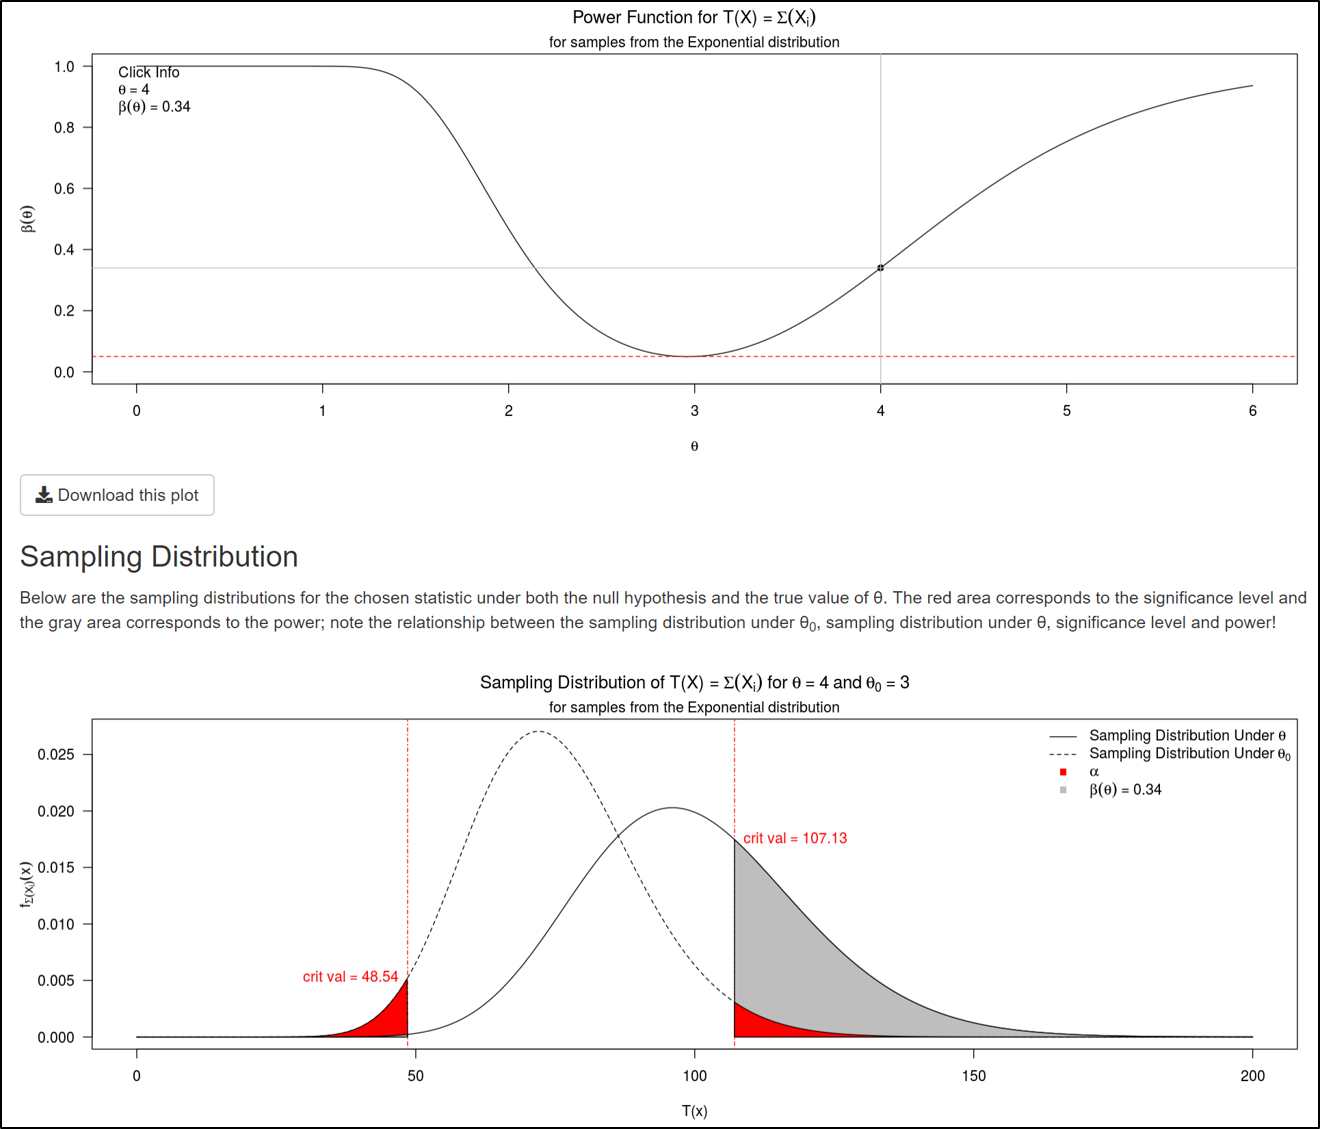
\includegraphics[scale=1]{reactive.png}
	\caption{Power function and associated sampling distributions for a hypothesis based on the sum of random variables for a sample of size 25 from the exponential distribution assuming a not equal to alternative hypothesis, significance level of 0.05, and null value of 3.}
\end{figure}

These explorations can also help students understand how power is determined from those distributions. In \hl{Figure 10}, the power is represented by the larger gray area and the significance level is represented by the smaller red area. From this graphic, students can visually assess how the significance level is used to determine the critical value, which is then used to calculate the power. Developing this conceptual understanding of how power is determined may help inform the derivation process for students and develop an intuition for how one might simulate power, which is further discussed in Section 3.3.

\subsection{Exploring other methods}

In the previous sections, we have largely focused on combinations of population distributions and statistics for which the distribution of the statistic is known in closed form and the power function is therefore readily obtainable. However this is not always the case when investigating power. In some cases, issues may arise that make it difficult to derive the formula for or visualize the power function. Learning how to resolve the issues that arise in these cases is valuable for students as it not only prepares them for potential challenges that they may encounter as a practicing statistician but also improves their ability to think critically and reason quantitatively. 

One issue a practicing statistician may encounter is that numerical instability in the distribution function of the statistic of interest. For example, even with modest sample sizes, the sampling distribution of the sum of uniform($0, \theta$) random variables exhibits numerical instability that manifests in the form of a strange oscillating pattern in the sampling distribution that is also visible in the power function (see \citealt{alberto2019} for more detail); this instability is exacerbated for larger sample sizes.  To understand this challenge, we first note that the distribution of the sum of independent uniform($0,1$) random variables is known as the Irwin-Hall($n$) distribution. It can be shown through transformation (Appendix A) that the distribution of the sum of uniform(0, $\theta$) random variables is a scaled form of the Irwin-Hall($n$) distribution, hereafter called the general Irwin-Hall($n, \theta$) distribution. The density function for this distribution is a piece-wise polynomial function (spline) of degree $n - 1$, where each piece of the spline can be represented by a power series with coefficients that alternate in sign. As a result, the density of this distribution at any point is numerically calculated by summing an alternating series. For density values close to zero or one, the precision with which the density can be calculated is limited by the precision of the statistical software used to plot the density function. This phenomenon is responsible for the aforementioned oscillating trend that may appear in the power function. 

The web application provides an opportunity to explore the issue of numerical instability. By clicking on the warning information that appears when the uniform distribution and sum of random variables is selected, students obtain additional plots and information {Figure 11}. The error message that appears allows students to zoom in on the numerical instability if the oscillating trend isn't obvious in the power function due to a small sample size. The message also describes two alternative ways to calculate the power of this test: through normal approximation using the Central Limit Theorem or through simulation. In the next two subsections, we explore how this web application may be used to explore each of these alternatives.

\begin{figure}[H]
	\centering
	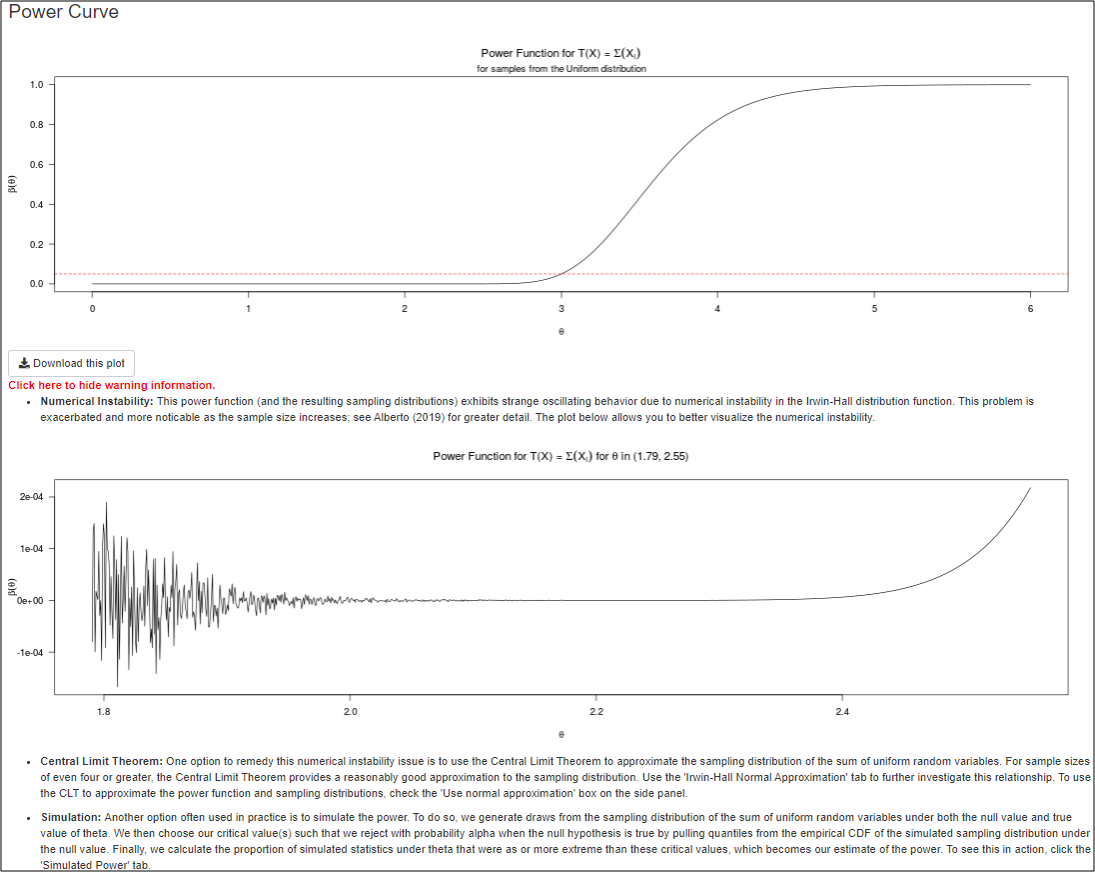
\includegraphics[width=\textwidth]{irwinerror.png}
	\caption{Toggleable error message notifying the user that numerical instability is present. The plot allows the user to ``zoom" in on the numerical instability, and the text proposes potential solutions.}
\end{figure}

\subsubsection{Exploring normal approximation}

The Central Limit Theorem is the first option the web application offers students to resolve the numerical instability issue. Through normal approximation, students can approximate the sampling distribution of the sum of uniform random variables and therefore the power function. To implement this solution, students click the ``Use normal approximation" check box that appears on the side panel for this combination of population distribution and statistic. Upon doing so, the power function and sampling distributions are replaced by those based on a normal approximation (\hl{Figure 12}).

\newpage

\begin{figure}[H]
	\centering
	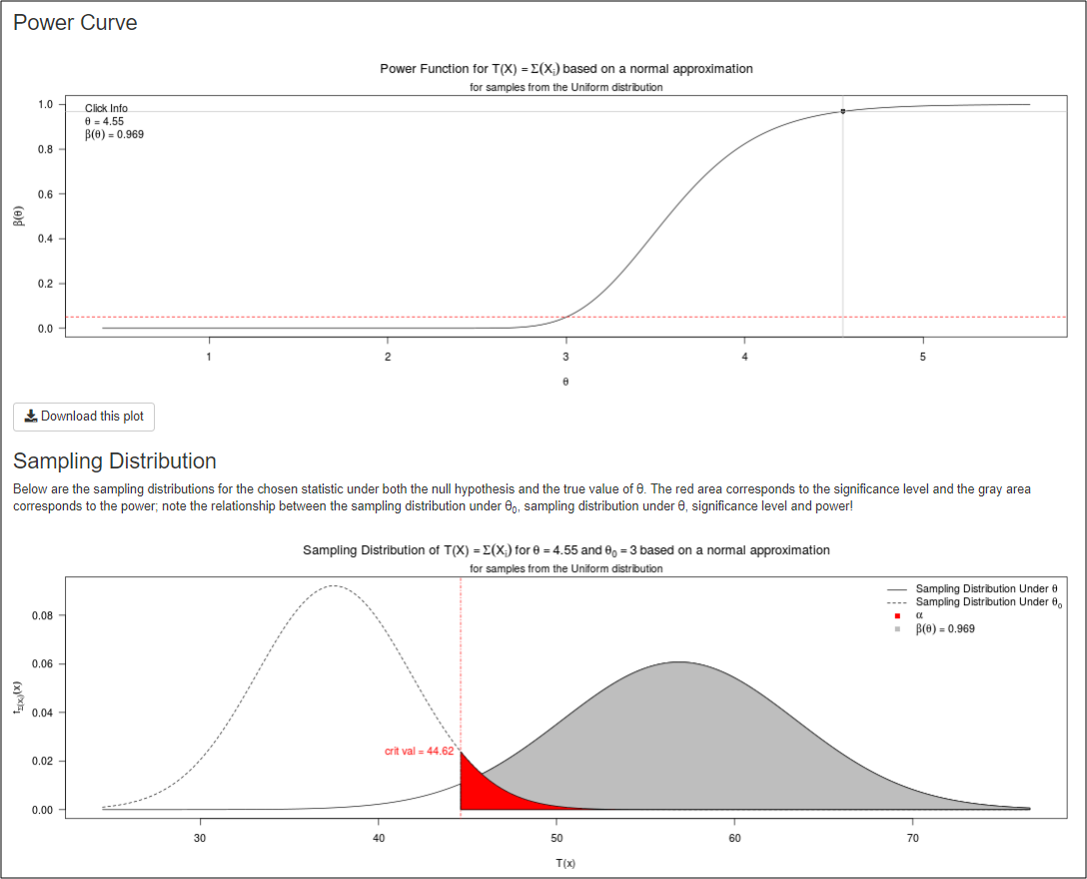
\includegraphics[width=\textwidth]{normapprox1.png}
	\caption{Power function and associated sampling distributions  for a test function based on the sum of random variables for samples from the uniform distribution assuming normal approximation through the Central Limit Theorem.}
\end{figure}

This exploration is valuable for students because it gives them an opportunity to use previously discussed tools to resolve a problem, as a practicing statistician would. The web application also gives students the option to evaluate how well the Central Limit Theorem approximates the sampling distribution of the sum of uniform random variables through the ``Irwin-Hall Normal Approximation" tab. In this tab, students may simulate many samples of a desired size from a uniform($0, \theta$) distribution by specifying the number of simulated samples, sample size, and value of $\theta$ in the sidebar. Students are then able to visualize the resulting empirical sampling distribution. Finally, students can assess the quality of the normal approximation by overlaying the approximate normal distribution function obtained through the Central Limit Theorem on the empirical distribution function (\hl{Figure 13}). 

The features this tab offers are beneficial because students can assess the quality of the approximation used to produce the power function for this test, similar to how one should when using the Central Limit Theorem in practice. The tab's features also demonstrate how flexible of a tool simulation can be when resolving difficult problems in statistics, which is further explored below. 

\begin{figure}[H]
	\centering
	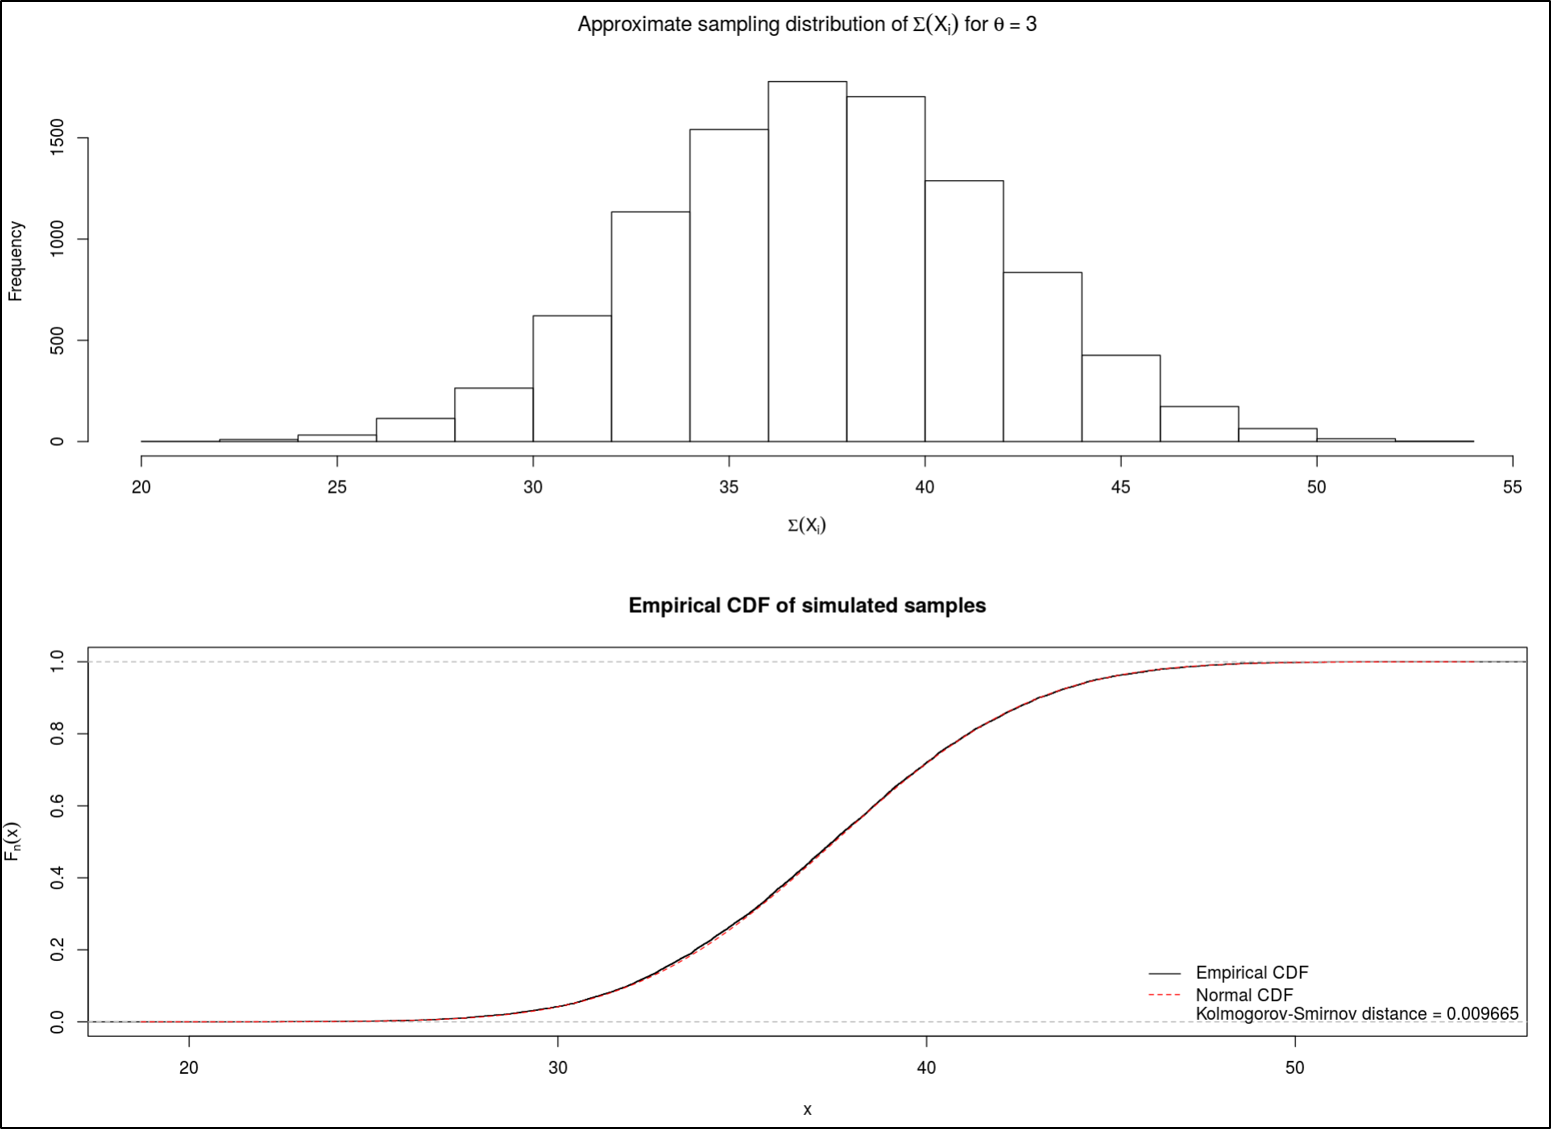
\includegraphics[width=\textwidth]{normapprox2.png}
	\caption{Diagnostic plots for the normal approximation using the Central Limit Theorem. The plot in the top row displays the approximate sampling distribution for the sum of random variables through a histogram and the bottom plot provides the empirical distribution function overlaid by the appropriate normal distribution function.}
\end{figure}

\subsubsection{Exploring simulation}

Students can also resolve the numerical instability issue by using simulation to approximate the sampling distribution of the sum of uniform random variables and the power function. The ``Simulated Power" tab offers a sidebar with options to specify the number of simulated samples, sample size, null value, significance level ($\alpha$), alternative hypothesis, and value of $\theta$. Once specified, students may click the ``Simulate power!" button to produce both the simulated power function and simulated sampling distributions under both the null value and the specified value of $\theta$ (\hl{Figure 14}).

To create the simulated power function, this web application first  creates a fine sequence of $\theta$ values along the x-axis. Then for each value of $\theta$, this web application simulates the specified number of simulated samples of the specified size from a uniform($0, \theta$) distribution and calculates the sum of simulated values for each of those samples (hereafter called the alternative sums); this process is repeated for the specified null value (hereafter called the null sums). Next, the critical value(s) is determined by calculating the $\alpha^{th}$ percentile of the null sums for a less than alternative, the $(1 - \alpha)^{th}$ percentile of the null sums for a greater than alternative, or the $(\alpha/2)^{th}$ and $(1 - \alpha/2)^{th}$ percentiles of the null sums for a not equal to alternative. Finally, the simulated power is determined by calculating the proportion of alternative sums that are as or more extreme than the corresponding critical values in the direction of the alternative hypothesis. The simulated power at each value of $\theta$ is then plotted against $\theta$ to produce the simulated power function. 

\begin{figure}[H]
	\centering
	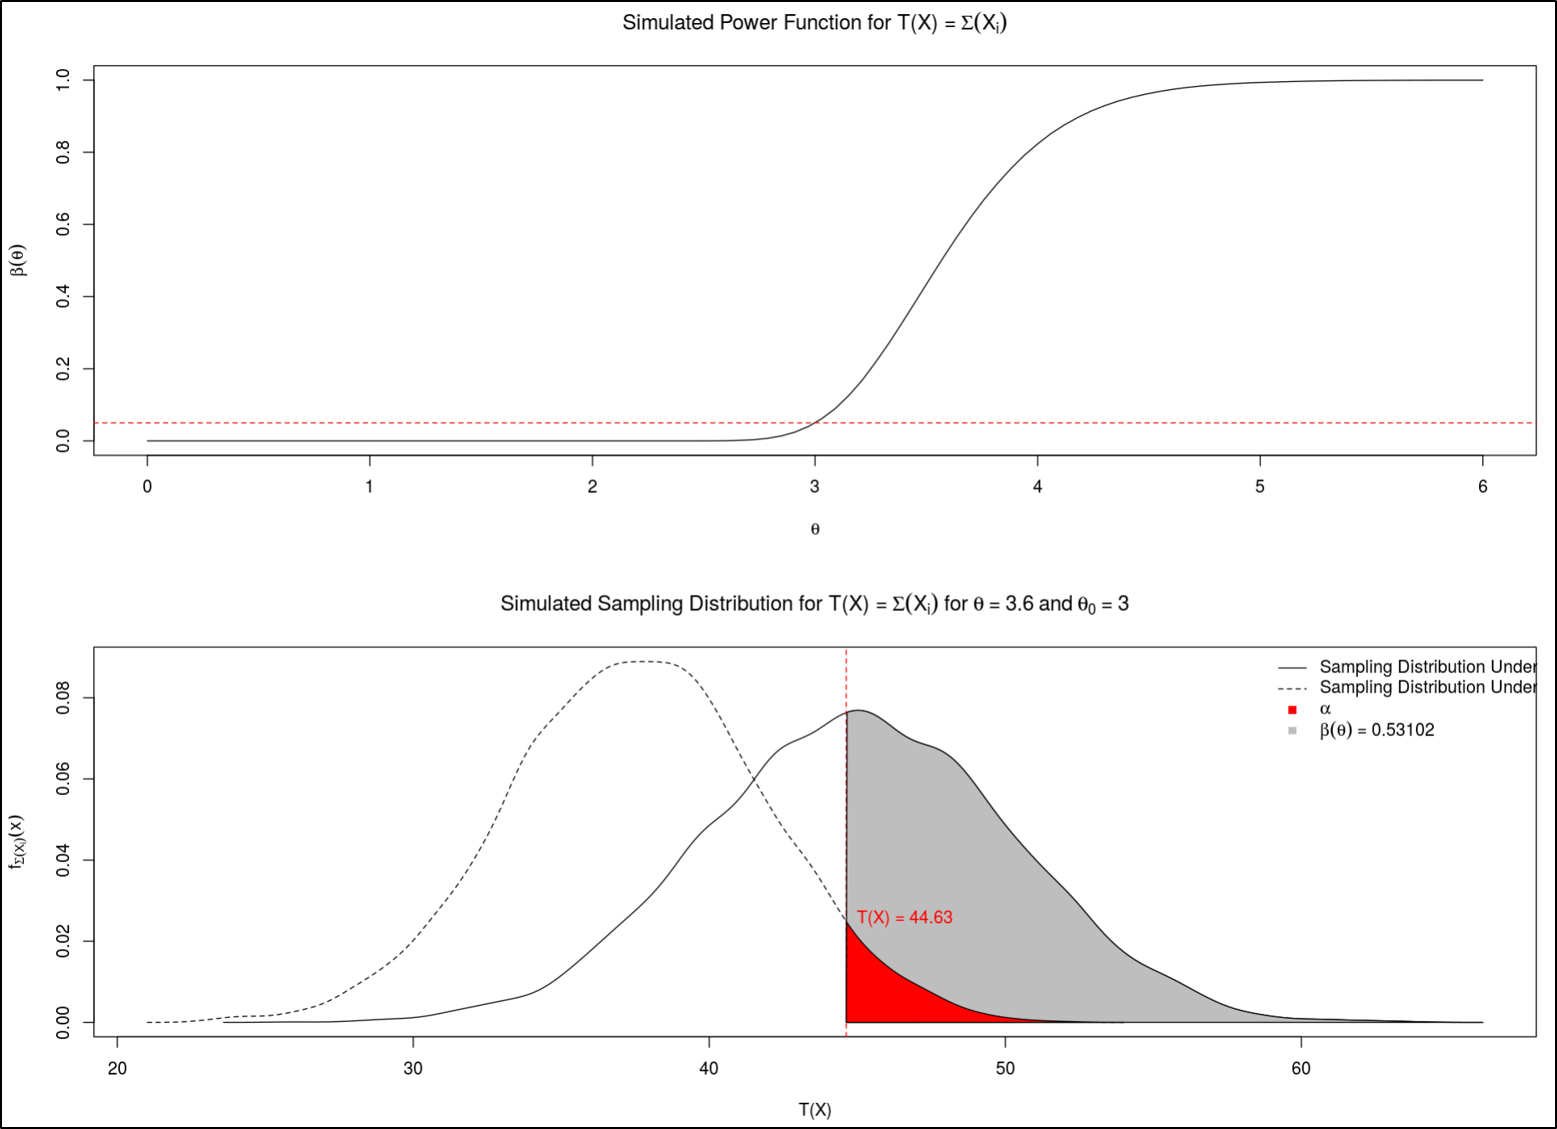
\includegraphics[width=\textwidth]{sim.png}
	\caption{Simulated power function and associated sampling distribution for a test based on the sum of random variables when sampling from a uniform population.}
\end{figure}
 
The simulated sampling distribution plot is created by repeating this process for only the value of $\theta$ specified on the sidebar and plotting the density of the resulting null and alternative sums. The shading is done by first determining the appropriate critical values as described above, then shading under each density in the appropriate direction as determined by the alternative hypothesis. The value of this process is two-fold for students. First, they are able to understand through application how powerful of a tool simulation can be for resolving complicated problems in Statistics. In many cases, practicing statisticians prefer simulation over analytical methods when conducting power analyses because of its flexibility and ease of implementation; this web application gives students the opportunity to witness this firsthand. Second, students develop a deeper conceptual understanding of the relationship between sampling distributions and power by considering how to simulate a power curve. Doing so requires stepping through the process described above, solidifying the understanding developed in the previous two sections. 

\section{APPLICATION IMPLEMENTATION}

We implemented this web application with a guided activity (see Appendix B) in three classes across two different semesters: (1) in the spring of 2018 with both an undergraduate-level and graduate-level mathematical statistics class and (2) in the spring of 2019 with a graduate-level mathematical statistics class. After each semester, the application was revised based on feedback provided by the students, offering additional population distributions, test statistics, alternative hypotheses, and features to explore (see Table 1), leading to its current form. In the following sections, we provide background information about the classes in which this application was implemented, describe the guided activity, and conclude with summaries of student reflections about the application. 

\begin{table}[H]
	\centering
	\begin{tabular}{|l|c|c|c|}
	\hline
	\thead{} & \thead{Version 1 \\ (Spring 2018)} & \thead{Version 2 \\ (Spring 2019)} & \thead{Version 3 \\ (Current, Spring 2020)} \\
	\hline
	Distributions & Exponential & \makecell{Exponential, uniform, \\ normal} & \makecell{Exponential, uniform, \\ normal} \\
	Statistics & \makecell{$\sum_{i=1}^n X_i$, $X_{(1)}$} & $\sum_{i=1}^n X_i$, $X_{(1)}$, $X_{(n)}$ & $\sum_{i=1}^n X_i$, $X_{(1)}$, $X_{(n)}$ \\[5mm]
	Alternatives & $<, >$ & $<, >, \neq$ & $<, >, \neq$ \\
	Additional features & None & Derivations tab & \makecell{Derivations tab, CLT \\ approximation tab, \\ simulation tab}\\
	\hline
	\end{tabular}
	\caption{Table of web application versions. Student feedback was used to revise each version of the application; version 3 is the current version described in Section 3 and is yet to be implemented.}
\end{table}

\subsection{Background context}

The application was used in the second semester of both an undergraduate-level and graduate-level two-semester sequence of courses in mathematical statistics. The first semester of each sequence of courses focuses on building the foundation of probability theory, addressing traditional topics such as probability, random variables, named probability distributions and multiple random variables. However, the graduate-level sequence of courses discusses these topics in greater depth, using the \cite{casella2002} text while the undergraduate-level sequence uses the \cite{wackerly2008} text. 

In the second semester, when this web application was implemented, the courses continue to address, such as sampling distributions, point estimation, hypothesis testing, and confidence interval estimation, but the graduate level course also covers asymptotics. In both courses, students discuss concepts of sufficiency and best unbiased estimation before investigating before investigating hypothesis testing and power during the last six weeks of the semester. 

Both the undergraduate and graduate level courses include students with diverse mathematics and statistics backgrounds, typically including students majoring in engineering, economics, and physics in addition to those seeking mathematics or statistics degrees. Prerequisites for the undergraduate level course include a course in multivariate calculus, with a course in mathematical proof also recommended. Prerequisites for the graduate level course include completion of the full undergraduate sequence (or a similar undergraduate sequence in mathematical statistics), though exceptions are made at the discretion of the instructor. In all three cases where this application was implemented, students were primed to use it by walking through a derivation of one of the power functions featured on the web application in the preceding class. In the following two 50 minute-long classes, students were asked to explore various properties of power using the web application through a guided activity, which is discussed in the next section. 

\subsection{Activity layout}

The same guided activity (Appendix B) was used across all three implementations, and was built around an example assuming an exponential population distribution. On the first day of each implementation, students were divided into five small groups and asked to explore one of the five questions provided in Part I of the activity. Students were then asked to summarize their group's exploration on a joint word document and give a short three to five minute presentation on what they discovered at the end of class. The structure of the second day differed between the undergraduate-level and graduate-level implementations. In the undergraduate-level course, the instructor lead an exploration of the relationship between the power function and sampling distribution using the web application at the beginning of class, after which students openly explored other relationships using the application. In the graduate-level implementations, students openly explored the relationship between the power function and sampling distribution for the first half of class and discussed what they discovered for the second half of class. In the spring 2019 implementation, students also explored additional population distributions which were newly available in that version of the application.

Following all three implementations, students were asked to answer a number of discussion questions (Appendix C). The spring 2019 cohort was asked an additional set of discussion questions related to the additional distribution and statistic options. These responses were used to guide a discussion at the beginning of class on the third day and clarify any lingering questions; the remainder of that third class was used to derive the power function for one of the examples provided on the web application. The student discussion question responses were also used to revise each version of the web application and assess the strengths and opportunities of the web application. We reviewed students' responses to these questions for each class at each implementation, summarizing the key points and paying special attention to comments about how the application helped or hindered there understanding of the material. Then, we compared these summaries across all three implementations to identify commonalities and differences between them. In the next section, we discuss the themes common to student responses at each implementation and provide some of our own reflections on this application's implementation. 

\subsection{Student reflections}

There were four types of comments common to all three implementations. The first type of comments consisted of descriptive statements about how the options on the sidebar panel influenced the power curve. These types of comments did not directly reference how the web application influenced their understanding of power, but instead provided indirect evidence of the web application's effect through descriptive statements. A student in the 2018 undergraduate cohort noted that ``the power function [varied] greatly depending on the test statistic used." Another student in the 2018 graduate cohort discovered that ``[as] the sample size increases, the power curve becomes steeper." There were many other similar comments describing fundamental relationship between the options available on the sidebar panel and the power curve. This type of feedback was very encouraging, as understanding those relationships is one of the learning objectives listed in Section 1. 

Across all three implementations, students also wrote about how the application allows them to quickly visualize changes in the power curve. Many students noted that the application's ability to render the power curve in real-time as they changed options on the side panel helped cement their understanding of the effect of each of those factors on the power curve. These comments provided direct feedback about how the application influenced their learning of power, as opposed to the indirect feedback discussed previously. A student in the 2018 undergraduate cohort stated that ``it was really helpful to be able to hold some inputs constant, while varying others and see how the power curve was affected." Another student in that cohort noted that it was helpful to ``change a parameter and immediately watch the distribution/power curve change with the parameter." Many students in the graduate cohorts echoed this sentiment. One student in the 2019 cohort felt that ``being able to adjust the things we control as researchers and seeing the instant feedback" was helpful. Overall, many students thought that being able to immediately visualize change in the power function and sampling distributions as they changed inputs on the side panel was helpful. 

In addition, students frequently described how the application helped them understand the role of the sampling distribution in calculating power as well as how the sampling distributions are used to determine the critical values of a test. Many students wrote that the web application helped them understand how the sampling distribution of a statistic is related to the power function and how the power function changes across statistics. For example, a student in the 2018 undergraduate cohort observed that ``the sampling distribution of $X_{(1)}$ hardly changes with increased sample size, so power does not really change for $X_{(1)}$ with increased sample size which is vice versa of the $\sum_{i=1}^n X_i$ statistic." Another student in that cohort noted that she ``really liked seeing the relationship between the null and observed sampling distributions... It really solidified the ideas behind power and critical values." Overall, students thought the visuals provided by this web application helped them understand different aspects of deriving a power function, including determining critical values. This understanding was mirrored in the graduate cohort. A student in the 2019 cohort described how she used the application to explore the relationship between sampling distributions and power in the following way:

\begin{quote}
	One aspect I found very helpful was being able to select various values of $\theta$ and seeing how this changed the sampling distribution. Not only did this connect power to the area under the distribution depending on $\alpha$ and $\theta$ but it also allowed us to make connections between power and the variance [of the test statistic]. 
\end{quote}

This type of feedback was again encouraging, as it suggested that this web application helped students better understand the relationship between the sampling distribution and the power curve, which is the second learning objective provided in Section 1. 

The final type of comments students frequently made focused on interesting relationships they noticed between the power function and previously discussed concepts. For example, students across all three cohorts noticed that power functions based on sufficient statistics tended to provide higher power across the alternative space than those based on other statistics. Two students in the 2018 undergraduate cohort noted that ``it is better to use a sufficient statistic to obtain higher power," and that ``when a sufficient statistic is used the power is higher in the alternative space." We again saw similar discussions in the graduate cohorts. One student in the 2018 cohort provided the following reflection:

\begin{quote}
	I find the relationship between complete, sufficient statistics and power intriguing. Are there ways to prove that maximum power is realized when using a complete, sufficient statistic? Is this always the case? For all alpha? In general, what is the relationship between complete, sufficient statistics, uniform minimum variance unbiased estimators, and power?
\end{quote}

The value in these student reflections is two-fold. It suggests that students are using this application to think critically about power and its relationship to previously discussed concepts and it also lays the foundation for comparing test functions, which is the topic that follows power. 

In addition to sufficiency, some students sought to explore other relationships. One student described his exploration in the following way:

\begin{quote}
	I also found exploring the `extreme' cases to be interesting. For example, what happens when our alternative value of $\theta$ is less than $\theta_0$, but we have a greater than alternative hypothesis? Interestingly, we still have power greater than 0 due to random chance.
\end{quote}

In this reflection, the student used the web application to understand why there is a positive probability of rejecting the null hypothesis over the null parameter space. This kind of feedback is indicative of the kind of insight students may gain by using this web application to explore their curiosities.

In the reflection questions, students were also asked to provide suggestions about how the web application could be improved. In the spring 2018 implementation, students in both the undergraduate-level and graduate-level courses noted that it would be useful to consider more population distributions, additional statistics, and to explore a not-equal-to alternative hypothesis. These suggestions led to the development of the second version of the web application, which added the normal and uniform distributions, sample maximum as a test statistic, and not-equal-to alternative hypothesis. When using this updated version in the spring 2019 implementation, students' comments then included distribution-specific observations. For example, one student noted that ``changing theta doesn't affect the variation of the normal distribution whereas it does affect the exponential distribution." This feedback was exciting to see, as it suggested that the additional options available in the second version of the web application helped students gain additional insight into what factors affect the power function. Another student from that cohort summarized this effect: ``[The additional options] helped me see that power curves don't always look similar and that changing the distribution will drastically change the form of $\beta(\theta)$." Students were again asked for suggestions to improve the web application in the 2019 implementation. There were few requests for changes to the web application, though one student did suggest additional distributions be added to the application, including discrete distributions; this a potential area of further work. We did add additional features to the web application after the spring 2019 implementation, including the normal approximation and simulation tabs. These features added additional flexibility for exploring and building connections across a variety of topics, including simulation, the Central Limit Theorem, and strategies for practicing statisticians when conducting power analyses. 

\section{CONCLUSIONS}

In this article, we described a web application that can be used to visualize many different aspects of power - such as the factors that affect power and the relationship between power and the sampling distributions of the test statistic across the null and alternative parameter spaces - for a variety of different population distributions and statistics. In doing so, class time typically spent on creating those visualizations can instead be used to allow students to explore the intricate relationships that make power so conceptually rich. This exploration provides students with a much more dynamic and authentic experience, as it does not depend on a subset of graphics created by either the student or the instructor \textit{a priori}. 

As evidenced by student feedback, this web application encourages students to develop a conceptual understanding of statistical power in which they can recognize the relationship between the power function and the sampling distribution of a statistic and draw connections between power and previously covered topics. We recommend this application be paired with a guided activity such as the one provided in Appendix B; additional questions that can be used to target specific aspects of power are provided in Appendix D. Readers may access a running version of the application at \url{https://powerapp.shinyapps.io/powerapp/}.

In the future, we intend to conduct further research into how this application influences students' learning of power, as well as into how other instructors adapt the application.  Source code for this application is provided on our GitHub page (available at [link removed for blinding]) so that others may tailor it to their own needs. By showcasing the flexibility and versatility of this web application in teaching power in a modern mathematical statistics curriculum, we hope others are encouraged to harness the power of technology when approaching conceptually difficult topics in their own curriculum. 

\newpage

\renewcommand\refname{\large 6. REFERENCES}
\bibliography{references}

\newpage

\begin{center}
	\textbf{\large 7. APPENDIX}
\end{center}

\begin{center}
	\textbf{\large A. General Irwin-Hall Distribution Derivations}
\end{center}


It can be shown that if $X_i \stackrel{iid}{\sim} \text{Unif}(0, 1)$ and we take a random sample of size $n$ from this population, then $Y = \sum_{i=1}^n X_i \sim \text{Irwin-Hall}(n)$ \citep{marengo2017}, where $Y$ has the following density and distribution functions:

\[
f_Y(y) = \begin{cases}
\frac{1}{(n-1)!} \sum_{k = 0}^{\left \lfloor{x}\right \rfloor} (-1)^k \binom{n}{k}(y-k)^{n-1}, \ y \in \mathbb{R} & 0 < y < n\theta \\
0 & \text{else}
\end{cases} 
\]

\[
F_Y(y) = \begin{cases}
0 & y < 0 \\
\frac{1}{n!} \sum_{k = 0}^{\left \lfloor{x}\right \rfloor} (-1)^k \binom{n}{k}(y-k)^{n} & 0 \leq y \leq n\theta \\
1 & y > n\theta 
\end{cases}
\]

We desire the distribution of the sum of $n$ independent, $\text{uniform}(0, \theta)$ random variables. If $W_i \stackrel{iid}{\sim} \text{Unif}(0, \theta)$, then $\sum_{i=1}^n W_i$ has the same distribution as $\theta Y$, where $Y \sim \text{Irwin-Hall}(n)$. Then for $T = \sum_{i=1}^n W_i$, 
\[
Pr(T \leq t) = Pr(\theta Y \leq t) = Pr\left(Y \leq \frac{t}{\theta}\right)
\]

Therefore, 
\[
\begin{split}
F_T(t) &= F_Y\left(\frac{t}{\theta} \right) \\
f_T(t) &= \frac{1}{\theta} f_Y\left(\frac{t}{\theta}\right)
\end{split}
\]

\newpage

\begin{center}
	\textbf{\large B. Power Application Activity}
\end{center}

\textbf{\underline{Objective}}: In this activity, each group is going to explore power curves and how these curves compare for different test statistics, null values, alternative hypotheses, alpha levels, and sample sizes. We will also explore how these functions arise, relating them to the sampling distribution of the test statistic.

\textbf{\underline{Context}}: Annual loss (in hundreds of dollars) is assumed to be an Exponential random variable with mean $\theta$. In a small metropolitan area, the average annual loss (in hundreds of dollars) due to theft has been assumed to be $\theta_0$. Suppose the police chief is interested in testing hypotheses about the mean annual loss. A random sample of $n$ annual losses due to theft is taken, and two hypothesis tests are proposed, one based on the test statistic, $X_{(1)}$, and one based on the test statistic, $\sum_{i=1}^n X_i$.  

\textbf{\underline{Directions}}: Use the power applet (\url{https://powerapp.shinyapps.io/powerapp/}) to explore the following questions. We will discuss questions 1-5 as a class and then dig deeper into our explorations with questions 6-7.

\begin{center}
	\hrule 
	\textbf{Part I: Varying Test Statistics, Null Values, Alternative Hypotheses, Alpha Levels, and Sample Sizes}
	\hrule
\end{center}

\begin{enumerate}
	\item[1)] Holding all other values constant, how does the power curve for a test based on the test statistic, $X_{(1)}$, compare to the power curve for a test based on the test statistic, $\sum_{i=1}^n X_i$? Why do you think this is the case?
	
	\vspace{1.5in}
	
	\item[2)] Holding all other values constant, what happens to the power curve as the null value changes? Why?
	
	\vspace{1.5in}
	
	\item[3)] Holding all other values constant, what happens to the power curve if the alternative hypothesis changes? Why?
	
	\vspace{1.5in}
	
	\item[4)] Holding all other values constant, what happens to the power curve as the alpha level changes? Why? 
	
	\vspace{1.5in}
	
	\item[5)] Holding all other values constant, what happens to the power curve as sample size changes? Why?
	
	\vspace{1.5in}
\end{enumerate}

\begin{center}
	\hrule
	\textbf{Part II: Connecting Power Curves to Sampling Distributions}	
	\hrule
\end{center}

\begin{enumerate}
	\item[6)] What is the power curve representing over the parameter space, $\Theta$? How is each point on the power curve obtained? To explore this, let's consider the following questions: \\
	
	\textbf{\underline{Scenario 1}}: Fix $\theta_0 = 3, \alpha = 0.05$, and $n = 25$ to test $H_1: \theta > \theta_0$ using the following test function: $\phi_S(\boldsymbol{X}) = \begin{cases}
	1 & \sum_{i=1}^n X_i > k \\ 0 & \text{else} \end{cases}$. 
	
	\begin{itemize}
		\item Click on the point on the power curve corresponding to $\theta = 3$. \\ 
		\begin{itemize}
			\item[$\circ$] Where is each sampling distribution centered? Why? \vspace{.5in}
			\item[$\circ$] What is $k$ for this situation? How is it determined? \vspace{.5in}
			\item[$\circ$] How does the power at $\theta = 3$ relate to the significance level? Why? \vspace{.5in}
		\end{itemize}
		\item What happens to the power when $\theta > 3$? Click on at least one more point on the power curve corresponding to a value of $\theta$ greater than 3. For each point, reflect on the following questions: \\
		\begin{itemize}
			\item[$\circ$] How does the sampling distribution used to calculate power at this value of $\theta$ change? \vspace{.5in}
			\item[$\circ$] What happens to the sampling distribution under $\theta_0$? \vspace{.5in}
			\item[$\circ$] What is $k$? How does this relate to the value of $k$ found earlier? Why? \vspace{.5in}
			\item[$\circ$] How is power calculated for this value of $\theta$? How does it compare to the significance level? Why? \vspace{.5in}
		\end{itemize}
		\item What happens to the power when $\theta < 3$? Click on at least one more point on the power curve corresponding to a value of $\theta$ less than 3. For each point, reflect on the following questions: \\
		\begin{itemize}
			\item[$\circ$] How does the sampling distribution used to calculate power at this value of $\theta$ change? \vspace{.5in}
			\item[$\circ$] What happens to the sampling distribution under $\theta_0$? \vspace{.5in}
			\item[$\circ$] What is $k$? How does this relate to the value of $k$ found earlier? Why? \vspace{.5in}
			\item[$\circ$] How is power calculated for this value of $\theta$? How does it compare to the significance level? Why? \vspace{.5in}
		\end{itemize}
		\item Why is power increasing as the distance between $\theta$ and $\theta_0$ increases over the alternative parameter space? Why is power decreasing as the distance between $\theta$ and $\theta_0$ increases over the null parameter space? \vspace{1in}
	\end{itemize}

	\textbf{\underline{Other Scenarios}}: Consider the questions for Scenario 1 for different scenarios of interest. What do you notice? How is each point on the corresponding power curve obtained? How does this differ across different scenarios?
	
	\vspace{3in}
	
	\item[7)] Relating back to your explorations earlier in questions 1-5, how do different values of the test statistic, null value, alternative hypothesis, alpha level, and/or sample size change the power curves? How does this relate to the sampling distribution of the test statistic? \vspace{2in}
\end{enumerate}

\newpage

\begin{center}
	\textbf{\large C. Discussion Questions}
\end{center}

The following discussion questions were asked of all students that used this web application in class. Note that only the students from the spring 2018 implementation - who had access to a version of the application that featured additional population distributions and statistics - were asked question 3. 

\begin{enumerate}
	\item[1)] What did you discover or notice as you explored how different values of the test statistic, null value, alternative hypothesis, alpha level, and/or sample size change the power curves, and how this all relates to the sampling distributions of the test statistics? \vspace{.5in}
	
	\item[2)] How did the applet for the exponential distribution help or hinder your understanding of power?
	\begin{itemize}
		\item What aspects of the applet were helpful? Why?
		\item What aspects weren't as helpful and/or could be improved? Why?
	\end{itemize} 

	\vspace{.5in}
	
	\item[3)] How did looking at other population distributions, statistics, and alternative hypotheses help or hinder your understanding about power?
	\begin{itemize}
		\item What aspects of this were helpful? Why?
		\item What aspects weren't as helpful and/or could be improved? How?
	\end{itemize}

	\vspace{.5in}

	\item[4)] What remaining questions or concerns do you have about power? \vspace{.5in}
\end{enumerate}

\newpage

\begin{center}
	\textbf{\large D. Additional Activity Questions}
\end{center}

We provide the following questions as additional resources to explore particular aspects of power in more detail.

\textbf{Varying the population distribution}

\begin{quote}
	\textit{Choose the sample maximum as the test statistic and greater than as the alternative hypothesis. Holding all other values constant, what happens to the power curve as the population distribution changes between exponential, normal, and uniform? Why?}
\end{quote}

\begin{quote}
	\textit{Which power function is closest to an ideal power curve? Why?}
\end{quote}

\textbf{Varying the test statistic}

\begin{quote}
	\textit{Choose the uniform distribution as the population distribution and not equal to as the alternative hypothesis. Holding all other values constant, compare the power functions for each of the available test statistics. Which statistic provides the highest power across the alternative space?}
\end{quote}

\begin{quote}
	\textit{Switch the population distribution to the normal distribution and repeat the previous exercise. Explain why your answer to each of these questions differs.}
\end{quote}

\textbf{Varying the alternative hypothesis}

\begin{quote}
	\textit{Choose the exponential distribution as the population distribution and sum of the X's as the statistic. Holding all other values constant, what happens to the power curve as the alternative hypothesis changes between greater than, less than, and not equal to? Why?}
\end{quote}

\begin{quote}
	\textit{Why is the power function not symmetric about the null value?}
\end{quote}

\begin{quote}
	\textit{Choose the uniform distribution as the population distribution, sample maximum as the statistic, not equal to as the alternative hypothesis, and set the sample size to one. Is this test unbiased? Why or why not?}
\end{quote}

\textbf{Varying the significance level}

\begin{quote}
	\textit{Choose any combination of population distribution and statistic. Holding all other values constant, what happens to the power function as the significance level increases? Why?}
\end{quote}

\begin{quote}
	\textit{Explain how the significance level affects the power curve in terms of the type I error rate. What trade-offs are made in terms of the probability of making a type II error when increasing the significance level? (Hint: recall that the power of a test is equal to one minus the probability of a type II error)}
\end{quote}

\textbf{Varying the null value}

\begin{quote}
	\textit{Choose any combination of population distribution and statistic. Holding all other values constant, what happens to the power function as you change the null value? Why does this happen?}
\end{quote}

\begin{quote}
	\textit{Explain the relationship between the power function, null value, and significance level.}
\end{quote}

\textbf{Varying n}

\begin{quote}
	\textit{Choose the normal distribution as the population distribution, sum of the X's as the test statistic, and not equal to as the alternative hypothesis. Holding all other values constant, what happens to the power function as the sample size increases? Why?}
\end{quote}

\begin{quote}
	\textit{Change the statistic to the sample minimum. What happens to the power function as the sample size increases?}
\end{quote}

\begin{quote}
	\textit{Why do you think the effect of the sample size on the power curve is lesser for the sample minimum than for the sum of the X's?}
\end{quote}

\textbf{Sampling distributions}

\begin{quote}
	\textit{Choose the exponential distribution as the population distribution, sum of the X's as the test statistic, greater than as the alternative hypothesis, a sample size of 25, and set the null value and theta to be three and four respectively. Describe where each of the distributions plotted under the Sampling Distribution heading is centered and what each distribution represents. Hint: recall that the distribution of the sum of $n$ exponential($\theta$) random variables is gamma($n, \theta$).}
\end{quote}

\begin{quote}
	\textit{Describe what the red and grey shaded areas represent. How is the red area used to determine the grey area?}
\end{quote}

\begin{quote}
	\textit{Which of the factors on the sidebar panel that affect each of these sampling distributions are controlled by the researcher and which are unknown? Based on your answer, how would you recommend a researcher increases the power of their hypothesis test?}
\end{quote}


\end{document}